%%%%%%%%%%%%%%%%%%%%%%%%%%%%%%%%%%%%%%%%%
% Beamer Presentation
% LaTeX Template
% Version 1.0 (10/11/12)
%
% This template has been downloaded from:
% http://www.LaTeXTemplates.com
%
% License:
% CC BY-NC-SA 3.0 (http://creativecommons.org/licenses/by-nc-sa/3.0/)
%
%%%%%%%%%%%%%%%%%%%%%%%%%%%%%%%%%%%%%%%%%

%----------------------------------------------------------------------------------------
%	PACKAGES AND THEMES
%----------------------------------------------------------------------------------------

\documentclass{beamer}

\mode<presentation> {

% The Beamer class comes with a number of default slide themes
% which change the colors and layouts of slides. Below this is a list
% of all the themes, uncomment each in turn to see what they look like.

%\usetheme{default}
%\usetheme{AnnArbor}
%\usetheme{Antibes}
%\usetheme{Bergen}
%\usetheme{Berkeley}
%\usetheme{Berlin}
%\usetheme{Boadilla}
%\usetheme{CambridgeUS}
%\usetheme{Copenhagen}
%\usetheme{Darmstadt}
%\usetheme{Dresden}
%\usetheme{Frankfurt}
%\usetheme{Goettingen}
%\usetheme{Hannover}
%\usetheme{Ilmenau}
%\usetheme{JuanLesPins}
%\usetheme{Luebeck}
\usetheme{Madrid}
%\usetheme{Malmoe}
%\usetheme{Marburg}
%\usetheme{Montpellier}
%\usetheme{PaloAlto}
%\usetheme{Pittsburgh}
%\usetheme{Rochester}
%\usetheme{Singapore}
%\usetheme{Szeged}
%\usetheme{Warsaw}

% As well as themes, the Beamer class has a number of color themes
% for any slide theme. Uncomment each of these in turn to see how it
% changes the colors of your current slide theme.

%\usecolortheme{albatross}
%\usecolortheme{beaver}
%\usecolortheme{beetle}
%\usecolortheme{crane}
%\usecolortheme{dolphin}
%\usecolortheme{dove}
%\usecolortheme{fly}
%\usecolortheme{lily}
%\usecolortheme{orchid}
%\usecolortheme{rose}
%\usecolortheme{seagull}
%\usecolortheme{seahorse}
%\usecolortheme{whale}
%\usecolortheme{wolverine}

%\setbeamertemplate{footline} % To remove the footer line in all slides uncomment this line
%\setbeamertemplate{footline}[page number] % To replace the footer line in all slides with a simple slide count uncomment this line

%\setbeamertemplate{navigation symbols}{} % To remove the navigation symbols from the bottom of all slides uncomment this line
}

\usepackage{todonotes}
\usepackage{graphicx} % Allows including images
\usepackage{booktabs} % Allows the use of \toprule, \midrule and \bottomrule in tables

%----------------------------------------------------------------------------------------
%	TITLE PAGE
%----------------------------------------------------------------------------------------
\newcommand\tab[1][1cm]{\hspace*{#1}}
\title[QALD]{QALD-Mini-Project} % The short title appears at the bottom of every slide, the full title is only on the title page

\author[Data Science]{Lukas Bl{\"u}baum \\ Nick D{\"u}sterhus \\ Ralf Keller} % Your name
\institute[UPB] % Your institution as it will appear on the bottom of every slide, may be shorthand to save space
{
University of Paderborn \\ % Your institution for the title page
\medskip
\textit{https://github.com/LukasBluebaum/QALD-Mini-Project} % Your email address
}
\date{July 19, 2018} % Date, can be changed to a custom date

\begin{document}

\begin{frame}
\titlepage % Print the title page as the first slide
\end{frame}

\begin{frame}
\frametitle{Overview} % Table of contents slide, comment this block out to remove it
\tableofcontents % Throughout your presentation, if you choose to use \section{} and \subsection{} commands, these will automatically be printed on this slide as an overview of your presentation
\end{frame}

%----------------------------------------------------------------------------------------
%	PRESENTATION SLIDES
%----------------------------------------------------------------------------------------

%------------------------------------------------
\section{Task Description} % Sections can be created in order to organize your presentation into discrete blocks, all sections and subsections are automatically printed in the table of contents as an overview of the talk

\begin{frame}
\frametitle{Task Description}
\begin{itemize}
	\item Building a Question Answering Engine that is able to get a F-measure of atleast 0.1 
	\item Using DBpedia as knowledge base
\end{itemize}
\begin{block}{Given}
\begin{itemize}
	\item Library qa.annotation (finding entities, properties, classes) and qa.commons (load / store QALD Datasets)
	\item A wrapper to plug in GERBIL QA
\end{itemize}
\end{block}
\end{frame}

%------------------------------------------------
\section{Our Approach}
%------------------------------------------------

\begin{frame}
\frametitle{Our Approach}
\begin{itemize}
	\item Template based
	\item Classify question types and apply natural language processing to get important keywords
	\item Find entities, classes, and properties that match the question
	\item Build SPARQL query templates for the most common types of questions 
\end{itemize}
\end{frame}

%------------------------------------------------
\section{Architecture}
%------------------------------------------------

\begin{frame}
\frametitle{Simplified Procedure}
\begin{center}
	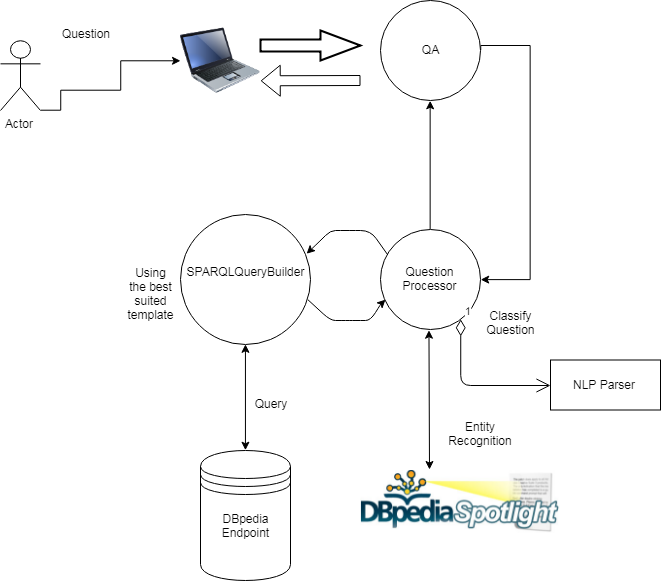
\includegraphics[scale=0.385]{Architecture.PNG}
\end{center}
\end{frame}

\begin{frame}
\frametitle{QA System}
\begin{itemize}
	\item Three modes:
	\begin{itemize}		
		\item Run offline: tries to answer one committed question
		\item Answer Dataset Questions: Load a QALD Dataset and save the result as a JSON-File (list of questions and their answers)
		\item Can be used as a webservice
	\end{itemize}
\end{itemize}
\end{frame}

\begin{frame}
	\frametitle{Webservice}
	\begin{itemize}
		\item Using the GerbilQA-Benchmarking-Template
		\begin{itemize}
			\item Webserver via the Spring Framework
			\item Takes a HTTP-POST request containing the question
		\end{itemize}
		\item Passes the question to the QuestionEngine
		\item Returns a JSON-String containing the answer and the used query
	\end{itemize}
\end{frame}

%------------------------------------------------
\section{Question Preprocessing}
%------------------------------------------------

\begin{frame}
\frametitle{Question Preprocessing}
\begin{itemize}
	\item Determining which method to build a sparql query should be applied
	\item Classifies questions by their starting word
	\begin{itemize}
		\item e.g. "When": we can conclude from that, that the given result should be from the datatype date or year
		\item Distinguish between ASK and SELECT clause
	\end{itemize}
\end{itemize}
\end{frame}

\begin{frame}
\frametitle{Question Preprocessing}
\begin{itemize}
	\item Requesting Spotlight to get all named entities in the question
	\item Using the Stanford CoreNLP to find keywords that give us information about the relations from the question 
	\item FindClasses/findProperties: Using IndexDBO\_classes from the qa.annotation library on nouns, verbs and adjectives
\end{itemize}
\end{frame}

%------------------------------------------------
\section{Template Overview}
%------------------------------------------------

\begin{frame}
\frametitle{Sparql Query Templates}
\begin{block}{Templates for different types of questions}
	\begin{itemize}
		\item Boolean questions such as: "Do Prince Harry and Prince William have the same parents?"
		\item List questions
		\item Who, Which, When, Where 
		\item How (much/many)
	\end{itemize}
\end{block}
\begin{itemize}
	\item Further differentiation which template to use based on number of classes/entities and comparison words
	\item Request DBpedia endpoint using Apache Jena library 
\end{itemize}
\end{frame}



\begin{frame}
\frametitle{Sparql Query Templates \\ {\normalsize Example Query}}
\begin{example}[most basic query]
	\begin{itemize}
		\item Question: "Who was the doctoral supervisor of Albert Einstein?"
		\item One Entity: Albert Einstein
		\item doctoral supervisor maps to property dbo:doctoralAdvisor  
		\item[] Query $\Rightarrow$ SELECT DISTINCT ?answer WHERE \{  \\
		\tab[1.4cm]	?answer a foaf:Person. 
		\tab[1.4cm] $<$http://dbpedia.org/resource/Albert\_Einstein$>$ 
		\tab[1.4cm] $<$http://dbpedia.org/ontology/doctoralAdvisor$>$ ?answer . \\
		\tab[1.4cm] \}
	\end{itemize}
\end{example}
\end{frame}

\begin{frame}
\frametitle{Sparql Query Templates \\ {\small Comparison}}
\begin{columns}[c] % The "c" option specifies centered vertical alignment while the "t" option is used for top vertical alignment
	
	\column{.5\textwidth} % Left column and width
	\begin{itemize}
		\item Predefined comparison enum for questions containing superlatives or comparatives
	\end{itemize}
	
	\column{.7\textwidth} % Right column and width
	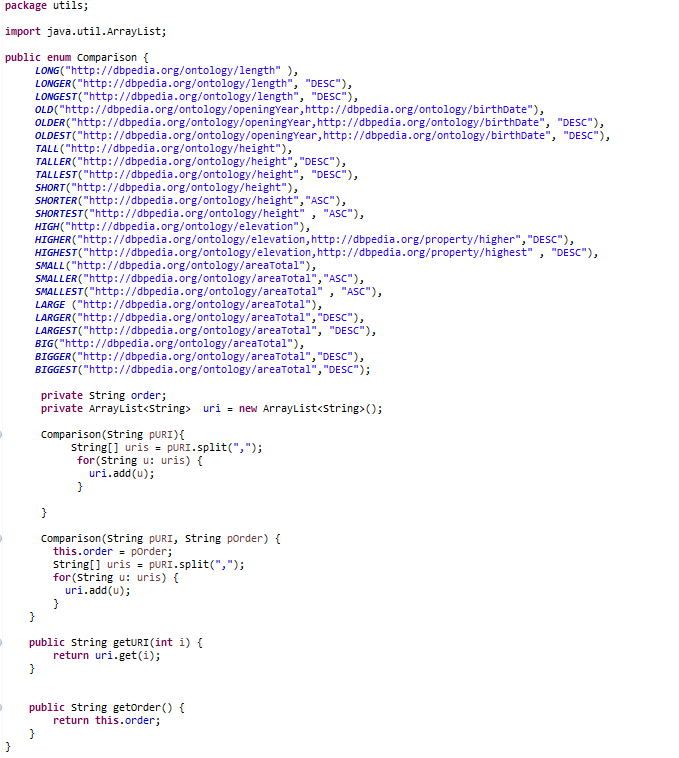
\includegraphics[scale=0.38]{Comparison.PNG}
	
\end{columns}
\end{frame}


\begin{frame}
\frametitle{Sparql Query Templates \\ {\normalsize Example Query}}
\begin{example}[largest]
	\begin{itemize}
		\item Question: "What is the largest country in the world?"
		\item Zero Entities
		\item One Class: Country
		\item Comparison enum: largest ( dbo:areaTotal )
		\item Order: DESC 
		\item Query $\Rightarrow$ SELECT ?answer WHERE \{ \\
		\tab[1.4cm] 	?answer rdf:type $<$http://dbpedia.org/ontology/Country$>$. 
		\tab[1.4cm] 	?answer  $<$http://dbpedia.org/ontology/areaTotal$>$ ?area .\} 
		\tab[1.4cm] 	ORDER BY DESC(?area) LIMIT 1 OFFSET 0

	\end{itemize}
\end{example}
\end{frame}


%------------------------------------------------
\section{Benchmarking}
%------------------------------------------------

\begin{frame}
\frametitle{Benchmarking \\ {\normalsize QALD8 Test}}
\begin{center}
	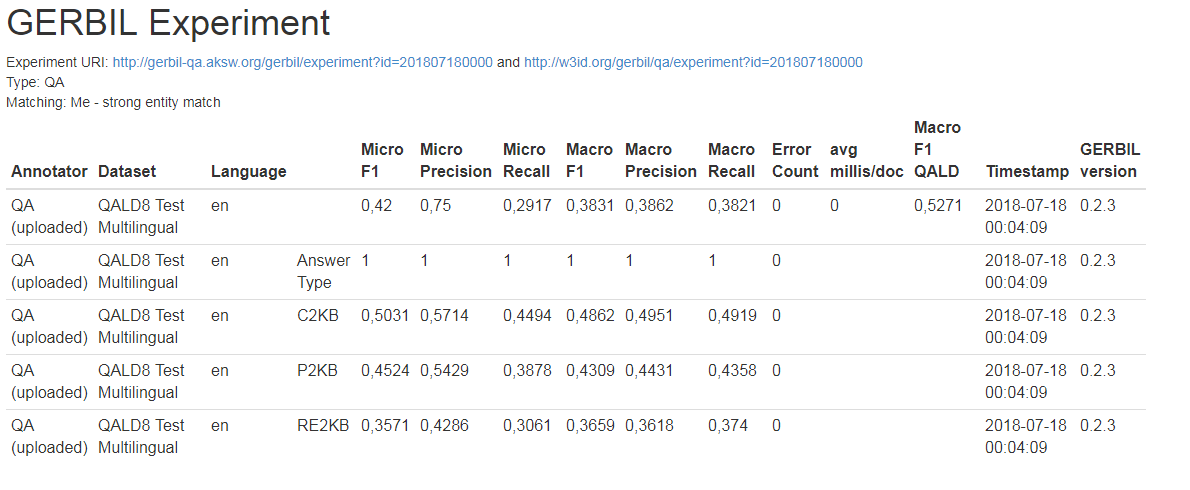
\includegraphics[scale=0.38]{QALD-8-Test.PNG}
\end{center}

\begin{itemize}
	\item  http://gerbil-qa.aksw.org/gerbil/experiment?id=201807160000
\end{itemize}
\end{frame}

\begin{frame}
\frametitle{Benchmarking \\ {\normalsize QALD8 Train}}
\begin{center}
	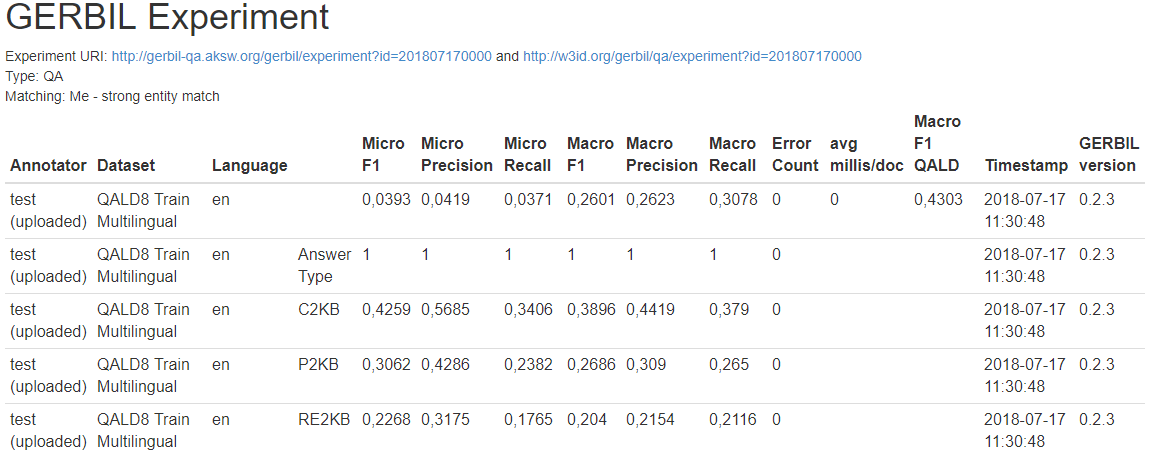
\includegraphics[scale=0.38]{QALD-8-Train.PNG}
\end{center}

\begin{itemize}
	\item  http://gerbil-qa.aksw.org/gerbil/experiment?id=201807170000
\end{itemize}
\end{frame}

\end{document} 